\documentclass[runningheads]{llncs}
\usepackage[T1]{fontenc}
\usepackage{graphicx}
\usepackage{amsmath,amssymb}
\usepackage{booktabs}
\usepackage{multirow}
\usepackage{url}

\begin{document}

\title{Amortized Explanation Distillation for Ultra-Low-Latency Fraud
Alerting: Trading Shapley Guarantees for Throughput on Real Ethereum
Transactions}

\titlerunning{Amortized Explanation Distillation for Fraud Alerting}

% TODO: replace with real author names / affiliations before submission
\author{First Author\inst{1} \and
Second Author\inst{1}}
\authorrunning{F. Author and S. Author}
\institute{Department of Computer Science, University Name, City, Country\\
\email{first.author@university.edu}}

\maketitle

\begin{abstract}
Payment platforms and blockchain-monitoring services score thousands of
events per second, yet the model-agnostic explainers regulators and
analysts rely on---KernelSHAP and LIME---cost tens of milliseconds
\emph{per explanation}, since each invocation requires hundreds of
auxiliary model evaluations. We study \emph{explanation distillation}:
training lightweight amortized neural surrogates
$g_\theta : x \mapsto \hat{\phi}(x)$ that map a transaction directly to its
predicted attribution vector in a single forward pass. On the real
Ethereum fraud-detection dataset (9{,}841 accounts, 22.1\% illicit), with a
gradient-boosting alert model (ROC-AUC $0.987 \pm 0.002$) and ten
independent seeds, distilled surrogates reproduce KernelSHAP attributions
with $R^2 = 0.870 \pm 0.025$, top-3 feature overlap $0.823 \pm 0.044$, and
Kendall $\tau = 0.688 \pm 0.020$, while reducing per-explanation latency
from $13.4$\,ms to under $5\,\mu$s---a $2{,}769\times$ speed-up
($4{,}262\times$ for LIME), i.e., throughput on the order of $10^5$
explanations per second on commodity CPUs. We characterise the full
amortization trade-off: fidelity as a function of teacher-set size, the
break-even point at which distillation beats direct explanation
($\approx 420$ explanations), and the price paid in Shapley-specific
guarantees, quantified as a local-accuracy (efficiency) gap of
$0.013 \pm 0.001$ probability mass---exactly zero for the teacher by
construction. The study provides deployment-oriented evidence that
faithful-enough explanations can be served at streaming rates, and
delineates precisely which theoretical properties are sacrificed.

\keywords{Explainable AI \and SHAP \and LIME \and Knowledge distillation
\and Amortized inference \and Fraud detection \and Ethereum \and
Low-latency systems.}
\end{abstract}

\section{Introduction}
Modern fraud-prevention systems operate under a dual mandate. On one side,
they must keep pace with transaction streams: card networks and
cryptocurrency-monitoring services evaluate thousands of events per second,
and risk decisions are taken within tight latency envelopes. On the other,
they face growing legal and operational pressure to \emph{explain} those
decisions---to analysts triaging alerts, to customers contesting blocks,
and to regulators auditing automated decision-making \cite{goodman2017}.

The de-facto standard explanation tools are model-agnostic: LIME
\cite{ribeiro2016} fits a local sparse linear surrogate from perturbation
responses, and KernelSHAP \cite{lundberg2017} estimates Shapley values
\cite{shapley1953} by regression over sampled feature coalitions. Their
model-agnosticism is bought with \emph{queries}: a single KernelSHAP
explanation with $n$ coalition samples requires $O(n \cdot |\mathcal{B}|)$
model evaluations against a background set $\mathcal{B}$, and LIME requires
$K$ perturbation queries plus a weighted regression. In our measurements on
a tuned gradient-boosting fraud model, this translates to
$13.4$\,ms (KernelSHAP, 300 coalitions) and $22.0$\,ms (LIME, 1{,}000
perturbations) per explanation on CPU---three to four orders of magnitude
slower than the classifier's own forward pass, and incompatible with
explaining every event in a high-volume alert stream.

A natural response is \emph{amortization}: spend the expensive computation
once, offline, on a \emph{teacher set} of exactly-computed explanations,
and distill it \cite{hinton2015,bucilua2006} into a small neural network
that maps a raw feature vector directly to its predicted attribution
vector. At serving time an explanation then costs one forward pass. This
idea underlies real-time saliency for images \cite{dabkowski2017},
information-theoretic explainer networks \cite{chen2018l2x},
supervised explanation models \cite{schwab2019}, and FastSHAP
\cite{jethani2022}, which trains an amortized Shapley estimator through a
weighted-least-squares objective. What is missing for the financial-fraud
setting is a \emph{deployment-oriented characterisation}: how much fidelity
does a plainly-engineered distilled surrogate achieve on real fraud data;
how does fidelity scale with the offline labelling budget; where is the
break-even point at which distillation is worth it; and---critically for
audit---\emph{which formal guarantees of the original explainers are lost},
and by how much?

This paper supplies that characterisation on the real Ethereum
fraud-detection dataset \cite{farrugia2020}, under a ten-seed protocol with
all results reported as mean $\pm$ standard deviation. Our contributions:
\begin{enumerate}
  \item An end-to-end distillation pipeline for both KernelSHAP and LIME
  over a gradient-boosting \cite{friedman2001} alert model, with surrogates
  that require no access to the explained model at serving time
  (Sect.~\ref{sec:method}).
  \item A quantified latency--fidelity frontier on real data:
  $2{,}769\times$ (SHAP) and $4{,}262\times$ (LIME) speed-ups at
  $R^2 = 0.87$ / $0.82$ and top-3 overlap $0.82$ / $0.79$ against the
  respective teachers, with full amortization curves over teacher budgets
  of 50--300 explanations and a measured break-even at roughly 420 served
  explanations (Sect.~\ref{sec:results}).
  \item An explicit audit of what distillation forfeits: the surrogate's
  Shapley local-accuracy (efficiency) gap is $0.013 \pm 0.001$ probability
  mass versus \emph{exactly zero} for KernelSHAP by construction, and sign
  fidelity concentrates on high-magnitude attributions---precisely the
  ones alert narratives are built from (Sect.~\ref{sec:discussion}).
\end{enumerate}

\section{Related Work}
\label{sec:related}

\subsubsection{Model-agnostic attribution.}
LIME \cite{ribeiro2016} and SHAP \cite{lundberg2017} dominate industrial
explainability practice; both are perturbation-driven and hence
query-expensive. Sampling-based Shapley estimation predates them
\cite{strumbelj2014}, and a substantial literature improves the estimator
itself: paired/antithetic sampling and regression refinements
\cite{covert2021_kshap}, dependence-aware value functions \cite{aas2021},
and, for tree ensembles, the polynomial-time TreeSHAP algorithm
\cite{lundberg2020}. These reduce constants but keep per-instance cost;
TreeSHAP is model-specific, and its interventional variant still scales
with background size. A recent survey of Shapley estimation trade-offs is
given by Chen et al.\ \cite{chen2023}.

\subsubsection{Amortized and real-time explanation.}
Dabkowski and Gal \cite{dabkowski2017} train a saliency-map generator for
images in real time; L2X \cite{chen2018l2x} learns an instance-wise feature
selector by maximising a mutual-information bound; CXPlain
\cite{schwab2019} trains a separate model to predict granger-style causal
importance with uncertainty estimates; FastSHAP \cite{jethani2022} learns
an amortized Shapley-value estimator by minimising the KernelSHAP
weighted-least-squares objective in expectation. Our work is complementary:
rather than proposing a new estimator, we perform a
regression-on-teacher-labels distillation---the variant simplest to deploy
and govern in regulated environments, since the teacher explanations
themselves can be archived for audit---and measure precisely what it buys
and costs on real fraud data, including the guarantee gap that
amortization introduces.

\subsubsection{Distillation.}
Knowledge distillation compresses a slow teacher into a fast student
\cite{bucilua2006,hinton2015}. We distill an \emph{explainer}, not a
classifier: the regression targets are attribution vectors, and the
relevant quality measures are rank-based (which features top the list)
rather than accuracy alone---hence our emphasis on top-$k$ overlap and
Kendall $\tau$ in addition to $R^2$.

\subsubsection{Fraud detection on Ethereum.}
Farrugia et al.\ \cite{farrugia2020} introduced the account-level Ethereum
illicit-account dataset used here and established gradient-boosting
baselines; broader anomaly-detection context is surveyed in
\cite{hilal2022}. Explanation reliability concerns---instability
\cite{alvarez2018} and adversarial manipulation \cite{slack2020}---apply to
teachers and surrogates alike and inform our stability-aware protocol.

\section{Methodology}
\label{sec:method}

Figure~\ref{fig:pipeline} gives an overview: an alert model produces a
stream of high-risk accounts; exact explainers label a teacher set offline;
amortized surrogates serve explanations online; and benchmarks quantify
latency, fidelity, and lost guarantees.

\begin{figure}[t]
\centering
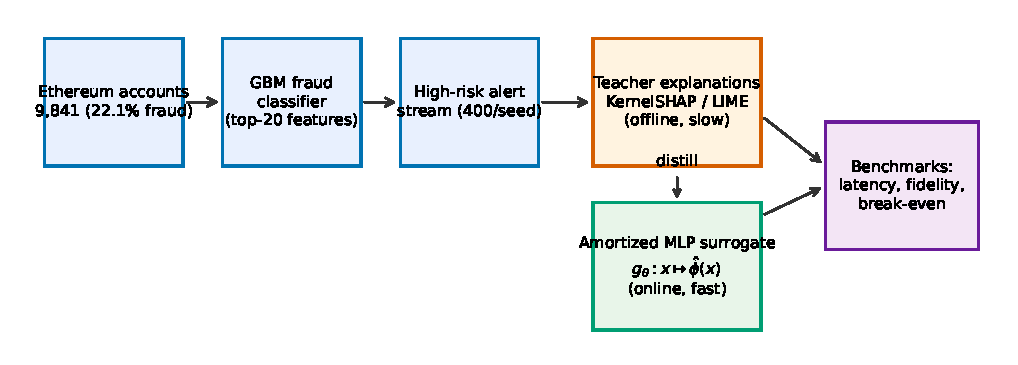
\includegraphics[width=\textwidth]{figures/fig0_pipeline.pdf}
\caption{Amortized explanation distillation. Expensive exact explainers run
offline on a teacher set of alerts; a lightweight surrogate
$g_\theta$ serves attribution vectors online in a single forward pass.}
\label{fig:pipeline}
\end{figure}

\subsection{Alert Model and Explanation Targets}
Let $f:\mathbb{R}^d \to [0,1]$ be a fraud classifier and
$x^\ast$ a flagged instance. KernelSHAP computes
$\phi^{\mathrm{SHAP}}(x^\ast) \in \mathbb{R}^d$ as the solution of the
weighted least-squares problem over coalitions $S$,
\begin{equation}
\min_{\phi}\;
\sum_{S \subseteq [d]} \pi(S)
\Bigl[v(S) - \phi_0 - \textstyle\sum_{j\in S}\phi_j\Bigr]^2,
\quad
v(S)=\mathbb{E}_{z\sim\mathcal{B}}\!\left[f\!\left(x^\ast_S \cup z_{\bar S}\right)\right],
\label{eq:kshap}
\end{equation}
with the Shapley kernel $\pi$ \cite{lundberg2017}; the solution satisfies
\emph{local accuracy} (efficiency),
\begin{equation}
\textstyle\sum_{j=1}^{d} \phi^{\mathrm{SHAP}}_j(x^\ast)
= f(x^\ast) - \mathbb{E}_{\mathcal{B}}[f],
\label{eq:efficiency}
\end{equation}
a property auditors can verify per explanation. LIME's attribution
$\phi^{\mathrm{LIME}}(x^\ast)$ is the coefficient vector of a locally
weighted sparse linear fit to $f$ over $K$ perturbations
\cite{ribeiro2016}. We use 300 coalition samples with a $k$-means
($k{=}10$) background for KernelSHAP and $K{=}1{,}000$ perturbations for
LIME.

\subsection{Amortized Surrogates}
For each explainer $E \in \{\mathrm{SHAP}, \mathrm{LIME}\}$ we collect a
teacher set
$\mathcal{T}_E = \{(x_i, \phi^{E}(x_i))\}_{i=1}^{n_t}$
of exactly-explained alerts and fit a multi-output regressor
\begin{equation}
\theta^\ast = \arg\min_\theta \frac{1}{n_t} \sum_{i=1}^{n_t}
\bigl\lVert g_\theta(x_i) - \tilde{\phi}^{E}(x_i) \bigr\rVert_2^2 ,
\label{eq:distill}
\end{equation}
where $\tilde{\phi}^{E}$ denotes per-dimension standardised targets
(statistics fitted on the teacher set and inverted at prediction time),
which stabilises optimisation given the heavy-tailed distribution of
attribution magnitudes. The surrogate is a two-hidden-layer perceptron
($128{\times}128$, ReLU, $\ell_2$ penalty $10^{-3}$), chosen deliberately
small: at serving time an explanation is one dense forward pass and, unlike
the teachers, requires \emph{no queries to $f$ at all}, decoupling
explanation serving from model-serving infrastructure.

\subsection{Evaluation Protocol}
\label{sec:protocol}
For each seed $\sigma \in \{0,\dots,9\}$: (i) split the data 70/30
(stratified); (ii) train the alert model; (iii) form an alert pool of the
400 highest-risk test accounts, mimicking the triage stream, and compute
teacher SHAP and LIME explanations for all of them, timing per-explanation
latency; (iv) randomly split the pool into 300 candidate teacher
explanations and 100 held-out evaluation alerts (random, to avoid
rank-induced covariate shift between training and evaluation); (v) train
surrogates on nested teacher subsets $n_t \in \{50, 100, 200, 300\}$ and
evaluate every surrogate on the same held-out 100 alerts.

\subsubsection{Fidelity metrics.}
Against the teacher on held-out alerts we report: mean-squared error and
$R^2$ over all attribution entries; \emph{sign agreement} (fraction of
entries with matching sign); \emph{top-3 overlap} between teacher and
surrogate feature rankings by $|\phi|$; and Kendall $\tau$ between
magnitude rankings. Rank-based metrics reflect how attributions are
actually consumed---as ordered reason lists in alert narratives.

\subsubsection{Guarantee gap.}
We measure the local-accuracy residual
$\Delta(x) = \bigl|\sum_j \hat\phi_j(x) + \phi_0 - f(x)\bigr|$
for teacher and surrogate SHAP; Eq.~\eqref{eq:efficiency} makes the teacher
residual zero up to solver tolerance, so $\Delta$ isolates what
amortization sacrifices.

\subsubsection{Systems metrics.}
Per-explanation latency (teacher vs.\ surrogate batch inference), surrogate
training time, and the break-even count
$N^\ast = (n_t \cdot \ell_T + t_{\mathrm{train}}) / (\ell_T - \ell_S)$,
where $\ell_T, \ell_S$ are teacher and surrogate latencies.

\section{Experimental Setup}
\label{sec:setup}

\subsubsection{Dataset.}
We use the public Ethereum fraud-detection dataset introduced by Farrugia
et al.\ \cite{farrugia2020}\footnote{\url{https://www.kaggle.com/datasets/vagifa/ethereum-frauddetection-dataset}}:
9{,}841 real Ethereum accounts (2{,}179 illicit, 22.14\%), each described
by aggregate transaction behaviour---timing statistics (e.g., average
minutes between sent/received transactions, lifetime span), volume counts
(sent/received/created contracts, unique counterparties), and Ether-value
statistics (min/max/avg sent, received, and contract-directed). After
removing identifiers and zero-variance columns, 38 numeric features remain;
per seed, the 20 most important by gradient-boosting split gain are
retained, keeping KernelSHAP's coalition space tractable
(Table~\ref{tab:setup}). No synthetic augmentation or resampling is
applied.

\begin{table}[t]
\centering
\caption{Experimental configuration (all results over 10 seeds).}
\label{tab:setup}
\begin{tabular}{lr}
\toprule
Property & Value \\
\midrule
Accounts / illicit rate & 9{,}841 / 22.14\% \\
Features after selection ($d$) & 20 (of 38 numeric) \\
Alert model & Gradient boosting (100 trees, depth 3) \\
Alert pool per seed & 400 top-risk test accounts \\
Teacher budgets $n_t$ & 50 / 100 / 200 / 300 \\
Held-out evaluation alerts & 100 per seed \\
KernelSHAP / LIME budget & 300 coalitions / 1{,}000 perturbations \\
Surrogate & MLP $128{\times}128$, target standardisation \\
Hardware & Commodity CPU (no GPU) \\
\bottomrule
\end{tabular}
\end{table}

\subsubsection{Alert-model quality.}
The gradient-boosting model attains ROC-AUC $0.987 \pm 0.002$ and average
precision $0.966 \pm 0.004$ on held-out accounts, consistent with the
strong ensemble baselines reported for this dataset \cite{farrugia2020};
the alert pool therefore consists of realistic, high-confidence fraud
flags.

\section{Results}
\label{sec:results}

\subsection{Latency and Throughput}
Table~\ref{tab:latency} and Fig.~\ref{fig:latency} give the headline
systems result. Exact per-explanation cost is $13.4 \pm 0.6$\,ms for
KernelSHAP and $22.0 \pm 0.8$\,ms for LIME; the distilled surrogates serve
attribution vectors in under $5\,\mu$s---speed-ups of
$2{,}769 \pm 307\times$ and $4{,}262 \pm 628\times$
respectively, i.e., throughput on the order of $2\times10^{5}$
explanations per second per CPU core, comfortably above payment-scale
alert volumes. Surrogate training itself is negligible
($1.6 \pm 0.4$\,s on 300 teacher examples).

\begin{table}[t]
\centering
\caption{Latency and speed-up (mean $\pm$ std over 10 seeds).}
\label{tab:latency}
\begin{tabular}{lccc}
\toprule
Explainer & Teacher latency & Surrogate latency & Speed-up \\
\midrule
KernelSHAP & $13.4 \pm 0.6$\,ms & $<5\,\mu$s & $2{,}769 \pm 307\times$ \\
LIME & $22.0 \pm 0.8$\,ms & $\approx 5\,\mu$s & $4{,}262 \pm 628\times$ \\
\bottomrule
\end{tabular}
\end{table}

\begin{figure}[t]
\centering
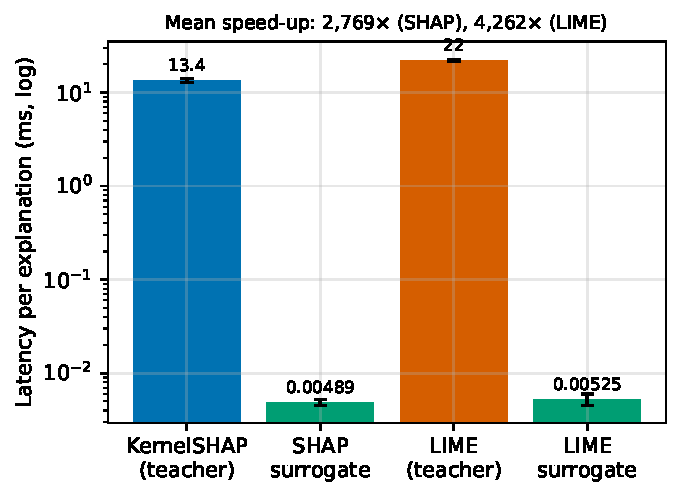
\includegraphics[width=0.62\textwidth]{figures/fig1_latency.pdf}
\caption{Per-explanation latency (log scale). Distillation moves
explanation serving from the tens-of-milliseconds regime to the
microsecond regime.}
\label{fig:latency}
\end{figure}

\subsection{Fidelity to the Teacher}
Table~\ref{tab:fidelity} and Fig.~\ref{fig:fdist} report fidelity at the
full teacher budget ($n_t{=}300$). The SHAP surrogate reproduces teacher
attributions with $R^2 = 0.870 \pm 0.025$ (MSE
$8.0\times10^{-4}$), ranks features with top-3 overlap
$0.823 \pm 0.044$ and Kendall $\tau = 0.688 \pm 0.020$; the LIME surrogate
achieves $R^2 = 0.820 \pm 0.038$, overlap $0.791 \pm 0.071$, and
$\tau = 0.527 \pm 0.049$. Figure~\ref{fig:scatter} visualises the
value-level agreement for SHAP across all seeds: predictions concentrate
tightly along the identity for high-magnitude attributions, with a Pearson
correlation of $0.93$ over every held-out attribution entry.

An instructive asymmetry appears in sign agreement: LIME's surrogate
matches signs on $75.0\%$ of entries, the SHAP surrogate on only
$48.9\%$---despite the SHAP surrogate's \emph{higher} $R^2$, overlap, and
$\tau$. The explanation is the distribution of targets: teacher SHAP
values on 20 features are overwhelmingly near-zero, where sign is
effectively noise, and the efficient allocation of Eq.~\eqref{eq:kshap}
spreads mass more sparsely than LIME's dense linear coefficients. Sign
fidelity conditional on magnitude is high precisely where it matters: the
top-ranked features that populate an alert narrative (cf.\ the tight
diagonal in Fig.~\ref{fig:scatter}). Rank-based metrics, not raw sign
agreement, are therefore the appropriate acceptance criterion for
distilled explainers.

\begin{table}[t]
\centering
\caption{Fidelity of surrogates to their teachers on 100 held-out alerts
per seed, at teacher budget $n_t = 300$ (mean $\pm$ std over 10 seeds).}
\label{tab:fidelity}
\begin{tabular}{lccccc}
\toprule
Surrogate & MSE & $R^2$ & Sign agr. & Top-3 overlap & Kendall $\tau$ \\
\midrule
SHAP & $0.0008 \pm 0.0002$ & $\mathbf{0.870 \pm 0.025}$ & $0.489 \pm 0.006$
& $\mathbf{0.823 \pm 0.044}$ & $\mathbf{0.688 \pm 0.020}$ \\
LIME & $0.0020 \pm 0.0004$ & $0.820 \pm 0.038$ & $\mathbf{0.750 \pm 0.015}$
& $0.791 \pm 0.071$ & $0.527 \pm 0.049$ \\
\bottomrule
\end{tabular}
\end{table}

\begin{figure}[t]
\centering
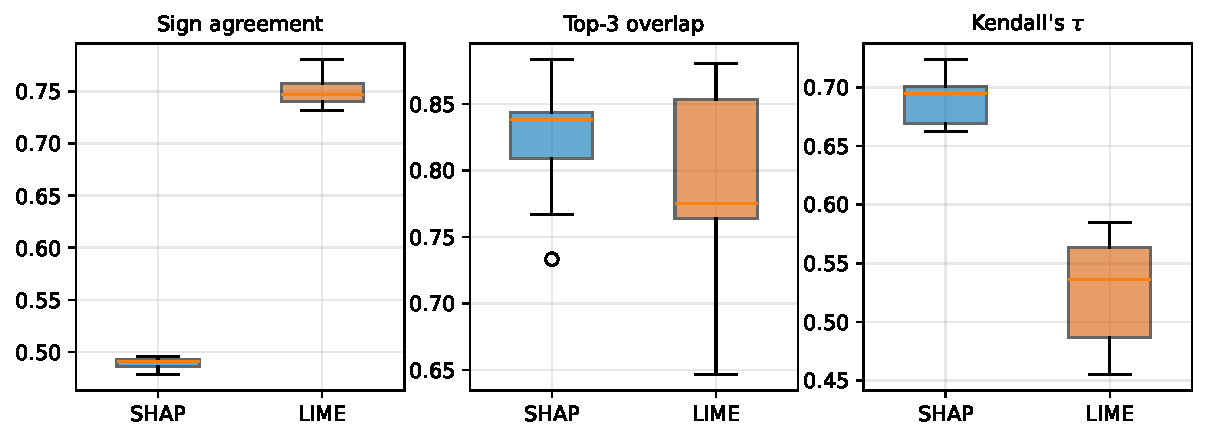
\includegraphics[width=0.95\textwidth]{figures/fig5_fidelity_dist.pdf}
\caption{Seed-level distribution of fidelity metrics at $n_t = 300$.}
\label{fig:fdist}
\end{figure}

\begin{figure}[t]
\centering

\includegraphics[width=0.55\textwidth]{figures/fig3_scatter.pdf}
\caption{Teacher KernelSHAP values vs.\ surrogate predictions on held-out
alerts, pooled over all 10 seeds (log-density hexbin). The dashed line is
the identity.}
\label{fig:scatter}
\end{figure}

\subsection{The Amortization Curve}
Figure~\ref{fig:amort} traces fidelity as the teacher budget grows.
Rank fidelity is remarkably budget-efficient: with only 50 teacher
explanations the SHAP surrogate already reaches top-3 overlap
$0.777 \pm 0.037$, rising to $0.823$ at 300. Value-level fidelity is the
budget-hungry component: $R^2$ climbs steeply from $0.44$ (SHAP) and
$-0.44$ (LIME) at $n_t{=}50$---where the LIME surrogate is unusable in
value terms---to $0.87$/$0.82$ at $n_t{=}300$, with variance shrinking
correspondingly. Deployments that consume only ranked reason lists can
therefore amortize with very small offline budgets, whereas any use of
attribution \emph{magnitudes} (e.g., thresholding contribution mass)
requires the larger teacher set.

\begin{figure}[t]
\centering

\includegraphics[width=\textwidth]{figures/fig2_amortization.pdf}
\caption{Fidelity vs.\ teacher budget $n_t$ (mean $\pm$ std over 10
seeds). Rank fidelity (left) saturates early; value fidelity (right)
requires the larger budgets.}
\label{fig:amort}
\end{figure}

\subsection{Break-Even Analysis}
Because distillation has a fixed offline cost---labelling $n_t$ teacher
alerts plus training---direct explanation is cheaper for small workloads.
With measured constants ($\ell_T = 13.4$\,ms, $\ell_S < 5\,\mu$s,
$t_{\mathrm{train}} = 1.6$\,s, $n_t = 300$), the total-cost curves cross at
$N^\ast \approx 420$ explanations (Fig.~\ref{fig:breakeven}); a fraud desk
serving more than a few hundred explanations amortizes its entire setup
within the first minutes of operation, after which every additional
explanation is effectively free relative to the direct baseline.

\begin{figure}[t]
\centering
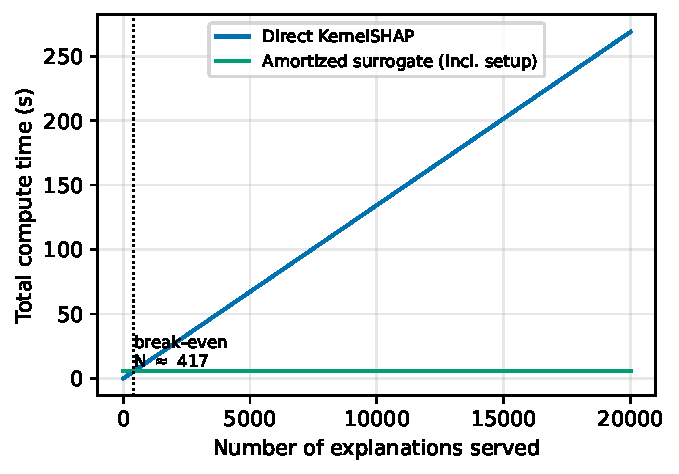
\includegraphics[width=0.62\textwidth]{figures/fig4_breakeven.pdf}
\caption{Cumulative compute of direct KernelSHAP vs.\ the amortized
surrogate (including teacher-labelling and training setup). The curves
cross at $N^\ast \approx 420$ served explanations.}
\label{fig:breakeven}
\end{figure}

\subsection{What Amortization Forfeits: the Guarantee Gap}
KernelSHAP's local-accuracy property (Eq.~\ref{eq:efficiency}) holds by
construction: we verify a residual of $0.000$ for every teacher
explanation. The distilled surrogate, being an unconstrained regressor,
inherits no such guarantee: its measured residual is
$\Delta = 0.013 \pm 0.001$ probability mass per alert. In audit terms, a
surrogate explanation's attributions sum to the model's output gap only
approximately---within about 1.3 percentage points of predicted fraud
probability on average. Institutions can (i) monitor $\Delta$ online as a
drift and quality signal at negligible cost, (ii) project surrogate
outputs onto the efficiency constraint by distributing the residual, or
(iii) escalate the small fraction of high-$\Delta$ alerts to the exact
teacher---a hybrid policy whose cost remains dominated by the surrogate
path.

\section{Discussion, Limitations, and Threats to Validity}
\label{sec:discussion}

\subsubsection{Deployment picture.}
The measured frontier supports a concrete architecture: exact explainers
run offline (and periodically, to refresh teachers under drift), an
amortized surrogate serves the alert stream at microsecond latency, and
the efficiency residual $\Delta$ plus periodic teacher audits provide the
governance signal. Because the surrogate never queries the alert model at
serving time, explanation capacity scales independently of model-serving
capacity---an operational property exact perturbation methods cannot
offer.

\subsubsection{Limitations.}
First, fidelity is measured \emph{to the teacher}: the surrogate is at
best as faithful to the model as KernelSHAP/LIME themselves, which have
known estimation error and manipulability \cite{slack2020,alvarez2018};
distillation adds a second approximation layer, and our guarantee-gap
metric quantifies only part of it. Second, the alert pool is
top-of-stream by design; surrogates trained on high-risk alerts should not
be assumed accurate on mid-distribution traffic without re-evaluation---we
mitigated the analogous pitfall \emph{within} the pool by randomising the
teacher/evaluation split, which proved essential (rank-ordered splits
inflate error severely through covariate shift). Third, results cover one
dataset, one tabular model class, and $d{=}20$ features; scaling behaviour
in $d$ and under concept drift, and comparison against
objective-amortized estimators such as FastSHAP \cite{jethani2022} and
uncertainty-aware explainers \cite{schwab2019}, are natural next steps.
Fourth, teacher refresh cost under non-stationarity is not modelled in the
break-even analysis; under drift, $N^\ast$ recurs per refresh cycle.

\subsubsection{Ethical note.}
Fast explanations can be consumed by adversaries probing a fraud model as
readily as by analysts; rate-limiting customer-facing explanation
endpoints and auditing for explanation-guided evasion remain necessary
regardless of serving speed.

\section{Conclusion}
Distilling KernelSHAP and LIME into small amortized surrogates converts
explanation from a tens-of-milliseconds perturbation procedure into a
microsecond forward pass. On real Ethereum fraud data, across ten seeds,
this preserved the consumable substance of explanations---feature
rankings ($0.82$ top-3 overlap, $\tau=0.69$) and attribution values
($R^2=0.87$)---at speed-ups of three-and-a-half orders of magnitude, with
a break-even under 500 served explanations and a quantified, monitorable
price: the loss of exact Shapley local accuracy, measured at
$1.3$ percentage points of probability mass. Faithful-enough explanation
at streaming throughput is thus practically attainable for fraud
alerting, provided rank-based acceptance criteria, randomized
teacher/evaluation protocols, and guarantee-gap monitoring accompany the
deployment.

\subsubsection{Reproducibility.} Code, per-seed raw results, and figure
scripts accompany this paper; the dataset is publicly available on Kaggle
\cite{farrugia2020}. Experiments use seeds $0$--$9$ throughout.

\begin{thebibliography}{25}

\bibitem{ribeiro2016}
Ribeiro, M.T., Singh, S., Guestrin, C.: ``Why should I trust you?'':
explaining the predictions of any classifier. In: Proc.\ 22nd ACM SIGKDD
International Conference on Knowledge Discovery and Data Mining,
pp. 1135--1144 (2016)

\bibitem{lundberg2017}
Lundberg, S.M., Lee, S.I.: A unified approach to interpreting model
predictions. In: Advances in Neural Information Processing Systems 30,
pp. 4765--4774 (2017)

\bibitem{shapley1953}
Shapley, L.S.: A value for $n$-person games. In: Contributions to the
Theory of Games II, pp. 307--317. Princeton University Press (1953)

\bibitem{jethani2022}
Jethani, N., Sudarshan, M., Covert, I., Lee, S.I., Ranganath, R.: FastSHAP:
real-time Shapley value estimation. In: Proc.\ 10th International
Conference on Learning Representations (ICLR) (2022)

\bibitem{schwab2019}
Schwab, P., Karlen, W.: CXPlain: causal explanations for model
interpretation under uncertainty. In: Advances in Neural Information
Processing Systems 32, pp. 10220--10230 (2019)

\bibitem{chen2018l2x}
Chen, J., Song, L., Wainwright, M.J., Jordan, M.I.: Learning to explain: an
information-theoretic perspective on model interpretation. In: Proc.\ 35th
International Conference on Machine Learning (ICML), pp. 883--892 (2018)

\bibitem{dabkowski2017}
Dabkowski, P., Gal, Y.: Real time image saliency for black box classifiers.
In: Advances in Neural Information Processing Systems 30, pp. 6967--6976
(2017)

\bibitem{farrugia2020}
Farrugia, S., Ellul, J., Azzopardi, G.: Detection of illicit accounts over
the Ethereum blockchain. Expert Systems with Applications \textbf{150},
113318 (2020)

\bibitem{friedman2001}
Friedman, J.H.: Greedy function approximation: a gradient boosting machine.
The Annals of Statistics \textbf{29}(5), 1189--1232 (2001)

\bibitem{lundberg2020}
Lundberg, S.M., Erion, G., Chen, H., DeGrave, A., Prutkin, J.M., Nair, B.,
Katz, R., Himmelfarb, J., Bansal, N., Lee, S.I.: From local explanations to
global understanding with explainable AI for trees. Nature Machine
Intelligence \textbf{2}(1), 56--67 (2020)

\bibitem{strumbelj2014}
\v{S}trumbelj, E., Kononenko, I.: Explaining prediction models and
individual predictions with feature contributions. Knowledge and
Information Systems \textbf{41}(3), 647--665 (2014)

\bibitem{covert2021_kshap}
Covert, I., Lee, S.I.: Improving KernelSHAP: practical Shapley value
estimation using linear regression. In: Proc.\ 24th International
Conference on Artificial Intelligence and Statistics (AISTATS),
pp. 3457--3465 (2021)

\bibitem{aas2021}
Aas, K., Jullum, M., L{\o}land, A.: Explaining individual predictions when
features are dependent: more accurate approximations to Shapley values.
Artificial Intelligence \textbf{298}, 103502 (2021)

\bibitem{chen2023}
Chen, H., Covert, I.C., Lundberg, S.M., Lee, S.I.: Algorithms to estimate
Shapley value feature attributions. Nature Machine Intelligence
\textbf{5}(6), 590--601 (2023)

\bibitem{hinton2015}
Hinton, G., Vinyals, O., Dean, J.: Distilling the knowledge in a neural
network. In: NIPS Deep Learning and Representation Learning Workshop
(2015), arXiv:1503.02531

\bibitem{bucilua2006}
Bucil\u{a}, C., Caruana, R., Niculescu-Mizil, A.: Model compression. In:
Proc.\ 12th ACM SIGKDD International Conference on Knowledge Discovery and
Data Mining, pp. 535--541 (2006)

\bibitem{alvarez2018}
Alvarez-Melis, D., Jaakkola, T.S.: On the robustness of interpretability
methods. In: ICML Workshop on Human Interpretability in Machine Learning
(2018), arXiv:1806.08049

\bibitem{slack2020}
Slack, D., Hilgard, S., Jia, E., Singh, S., Lakkaraju, H.: Fooling LIME and
SHAP: adversarial attacks on post hoc explanation methods. In: Proc.\
AAAI/ACM Conference on AI, Ethics, and Society (AIES), pp. 180--186 (2020)

\bibitem{goodman2017}
Goodman, B., Flaxman, S.: European Union regulations on algorithmic
decision-making and a ``right to explanation''. AI Magazine
\textbf{38}(3), 50--57 (2017)

\bibitem{hilal2022}
Hilal, W., Gadsden, S.A., Yawney, J.: Financial fraud: a review of anomaly
detection techniques and recent advances. Expert Systems with Applications
\textbf{193}, 116429 (2022)

\bibitem{molnar2022}
Molnar, C.: Interpretable Machine Learning: A Guide for Making Black Box
Models Explainable, 2nd edn. (2022), \url{https://christophm.github.io/interpretable-ml-book}

\end{thebibliography}

\end{document}
